\documentclass[12pt]{article}
\usepackage[utf8]{inputenc}
\usepackage[T1]{fontenc}
\usepackage{amsmath, amssymb}
\usepackage{geometry}
\usepackage{tikz}
\usepackage{hyperref}
\geometry{margin=1in}

\title{\Huge \textbf{Beyond the Known: A Unified Theory of Cognitive Limits} \\ 
\large \textit{The Emergent Network of Unsolved Problems and Axiom 13}}
\author{Teodor Berger}
\date{May 13, 2025}

\begin{document}

\maketitle

\begin{center}
\textit{Dedicated to those who dare to think beyond the known — where the unsolved becomes the frontier.}
\end{center}

\vspace{1cm}

\section*{Abstract}
This essay presents the Cognitive Frontier Theory (CFT), a framework uniting 20 top unsolved problems—10 mathematical (e.g., Riemann Hypothesis) and 10 physical (e.g., Nature of Time)—into an emergent network defined by a collective cognitive limit. We propose that current scientific methods (\(\Pi_{\text{curent}}\), the current scientific paradigm) cannot resolve these, requiring a new paradigm (\(\Pi_{\text{new}}\)). Inspired by Axiom 13 (DOI: \href{https://doi.org/10.5281/zenodo.15398105}{10.5281/zenodo.15398105}), we explore how ignoring the present day mirrors these limits, suggesting a global shift in logic, language, and validation, and glimpse AI’s future role.

\section*{Introduction}
Science thrives on challenges, and these 20 problems are its greatest peaks. Ten are mathematical giants—like the Riemann Hypothesis and P vs NP—and ten are physical mysteries—such as quantum gravity and dark matter. Rather than isolated puzzles, they form a network of barriers shaped by what today’s paradigm \(\Pi_{\text{curent}}\)—the set of methods and concepts we use to understand the world—cannot grasp. This essay introduces the Cognitive Frontier Theory (CFT), arguing for a shared cognitive root among these problems. We map their interconnections, propose a new framework to transcend these limits, and link it to Axiom 13, a playful exploration of ignoring the present day, which mirrors the broader challenge of understanding time itself.

\section*{The 20 Unsolved Problems: A Snapshot}
Here are the 20 unsolved problems, with mathematical challenges on the left and physical mysteries on the right:

\begin{center}
\begin{minipage}{0.48\textwidth}
\raggedright
\textbf{Top 10 Math Problems}
\begin{enumerate}
  \item Riemann Hypothesis
  \item Goldbach Conjecture
  \item Birch–Swinnerton-Dyer Hypothesis
  \item Hodge Conjecture
  \item P vs NP
  \item Navier–Stokes Regularity
  \item Generalized Poincaré Conjecture
  \item Collatz Conjecture
  \item Langlands Program
  \item Extended Four-Color Problem
\end{enumerate}
\end{minipage}
\begin{minipage}{0.48\textwidth}
\raggedright
\textbf{Top 10 Physics Problems}
\begin{enumerate}
  \item Quantum Gravity
  \item Dark Matter/Energy
  \item Hierarchy Problem
  \item Grand Unification
  \item Quantum Black Holes
  \item Dark Matter Particle
  \item Cosmic Origin
  \item CP Violation
  \item Turbulence
  \item Nature of Time
\end{enumerate}
\end{minipage}
\end{center}

\section*{The Cognitive Frontier Theory (CFT)}
These 20 problems form an emergent network \(S\), where each problem \(P_i\) (\(i=1,\dots,20\)) is a node on the boundary of our knowledge—the \emph{cognitive limit}—defined by \(\Pi_{\text{curent}}\), the current scientific paradigm encompassing today’s logic, language, and methods. Solving them demands \(\Pi_{\text{new}}\), a future paradigm with a redefined approach.

\subsection*{The Emergent Network}
{\sloppy
Nodes \(P_i\) are connected by relations \(R_{ij}\) when they share deep conceptual structures. For example, the concept of infinity links the Riemann Hypothesis (\(P_1\)) and the Nature of Time (\(P_{20}\)).
}
Below, we visualize a simplified portion of \(S\):
\begin{figure}[ht]
  \centering
  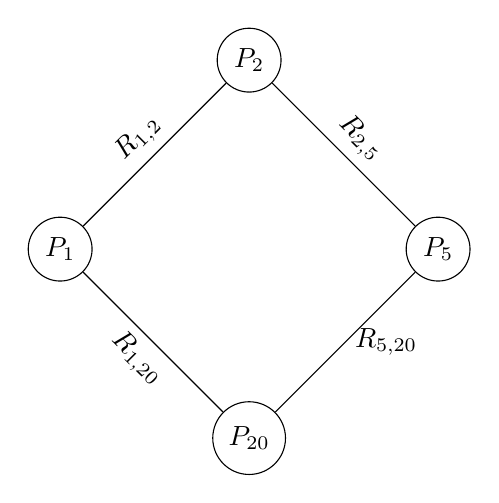
\begin{tikzpicture}[scale=1.2]
    \node[circle,draw] (P1) at (0,0) {$P_1$};
    \node[circle,draw] (P2) at (2,2) {$P_2$};
    \node[circle,draw] (P5) at (4,0) {$P_5$};
    \node[circle,draw] (P20) at (2,-2) {$P_{20}$};
    \draw (P1) -- (P2) node[midway,above,sloped] {$R_{1,2}$};
    \draw (P2) -- (P5) node[midway,above,sloped] {$R_{2,5}$};
    \draw (P5) -- (P20) node[midway,right] {$R_{5,20}$};
    \draw (P1) -- (P20) node[midway,below,sloped] {$R_{1,20}$};
  \end{tikzpicture}
  \caption{Network \(S\) with nodes representing unsolved problems: \(P_1 =\) Riemann Hypothesis, \(P_2 =\) Goldbach Conjecture, \(P_5 =\) P vs NP, \(P_{20} =\) Nature of Time. Relations \(R_{ij}\) indicate shared concepts (e.g., \(R_{1,20}\): infinity).}
  \label{fig:network}
\end{figure}

\subsection*{Mathematical Framework}
To quantify how far each problem lies beyond \(\Pi_{\text{curent}}\), we define an \emph{emergence index} \(E(P_i)\):
\begin{equation}
  \label{eq:emergence_index}
  E(P_i) = C(P_i) \cdot \log(|R_{ij}|) \cdot \text{dist}(P_i, \Pi_{\text{curent}})
\end{equation}

\vspace{0.2cm}
Here:
\begin{itemize}
  \item \(C(P_i)\): Complexity, estimated from computational or theoretical efforts (e.g., \(C(\text{Riemann}) \approx 10^{10}\), based on numerical checks of zeta zeros).
  \item \(|R_{ij}|\): Number of connections to other problems (e.g., Riemann has \(\sim 5\) links to physics and math problems via infinity and computation).
  \item \(\text{dist}(P_i, \Pi_{\text{curent}})\): Distance from the current paradigm, a value in [0,1] (e.g., 0.9 for hard problems, indicating they are far from current methods).
\end{itemize}

\vspace{0.2cm}
\textit{Note: \(E(P_i)\) is a novel, original proposal by the author to quantify the emergent nature of these problems. The logarithm \(\log(|R_{ij}|)\) reflects the natural scaling of interconnectedness, ensuring the index grows appropriately with the network’s complexity.}

\vspace{0.2cm}
Example: For the Riemann Hypothesis, \(C \approx 10^{10}\), \(|R_{ij}| \approx 5\), \(\text{dist} \approx 0.9\), so:
\[
E(\text{Riemann}) = 10^{10} \cdot \log(5) \cdot 0.9 \approx 6.3 \times 10^{10}.
\]

\subsection*{The New Paradigm \(\Pi_{\text{new}}\)}
To transcend \(\Pi_{\text{curent}}\), \(\Pi_{\text{new}}\) must include:
\begin{itemize}
  \item \textbf{Logic}: A hybrid of quantum and constructive logic, allowing for non-classical reasoning.
  \item \textbf{Language}: Based on symmetries, such as Lie groups, which are foundational in both mathematics (Langlands Program) and physics (String Theory).
  \item \textbf{Validation}: Combined theoretical-experimental methods, such as quantum simulations and numerical verifications.
\end{itemize}

\section*{Axiom 13: A Case Study}
Axiom 13 (DOI: \href{https://doi.org/10.5281/zenodo.15398105}{10.5281/zenodo.15398105}) explores the paradox of ignoring the present day when counting time intervals. This playful idea mirrors the cognitive limits in \(S\), particularly for \(P_{20}\) (Nature of Time). Ignoring today reflects a failure of \(\Pi_{\text{curent}}\) to fully grasp temporal structures, suggesting that \(\Pi_{\text{new}}\) must redefine how we conceptualize and model time in both mathematics and physics.

\section*{The Future: AI’s Role in Breaking the Frontier}
AI and quantum computing could accelerate progress beyond \(\Pi_{\text{curent}}\). For instance, in 2023, AI models like AlphaCode generated hypotheses for Riemann zeros, though not sufficient for a proof. Similarly, deep learning could detect dark matter patterns by analyzing cosmic microwave background data. AI’s ability to explore non-human reasoning patterns offers a path toward \(\Pi_{\text{new}}\), potentially uncovering new logical frameworks or simulating complex physical systems like quantum gravity.

\section*{Conclusion and Outlook}
CFT casts the 20 unsolved problems as an emergent network on our cognitive frontier. Their resolution requires a global shift in scientific logic, language, and validation—guided by insights from Axiom 13 and empowered by AI. This journey beyond the known is our next scientific leap, inviting us to redefine how we understand the universe and its fundamental structures.

\section*{References}
\begin{itemize}
  \item Riemann, B. (1859). “Ueber die Anzahl der Primzahlen unter einer gegebenen Grösse.” \textit{Monatsberichte der Berliner Akademie}.
  \item Witten, E. (1995). “String Theory Dynamics in Various Dimensions.” \textit{Nuclear Physics B}, 443.
  \item Gödel, K. (1931). “Über formal unentscheidbare Sätze der Principia Mathematica und verwandter Systeme I.” \textit{Monatshefte für Mathematik und Physik}, \href{https://doi.org/10.1007/BF01700692}{DOI: 10.1007/BF01700692}.
\end{itemize}

\end{document}
